\documentclass[aspectratio=169,11pt]{beamer}
\graphicspath{{figures/}} % Setting the graphicspath

% Theme settings
\usetheme{Madrid}
\usecolortheme{default}
\setbeamertemplate{navigation symbols}{}   % removes navigation symbols such as 'next page'
\setbeamertemplate{footline}{}             % remove line with name, date, page nr. 
\setbeamercolor*{frametitle}{bg=white}     % remove background from frametitle
\usepackage{caption}
% \captionsetup[figure]{labelformat=empty}% redefines the caption setup of the figures environment in the beamer class.
\setbeamersize{text margin left=20pt,text margin right=10pt}

\usefonttheme[onlymath]{serif} % makes beamer math look like article math


%======================= import packages =======================
\usepackage{graphicx}     % More options for \includegraphics
\usepackage{appendixnumberbeamer} % separate appendix numbering
\usepackage{hyperref}


%======================= page numbering =======================
\addtobeamertemplate{navigation symbols}{}{ \usebeamerfont{footline}
  \insertframenumber / \inserttotalframenumber \hspace*{2mm} \\ \vspace*{1mm} 
}


%=================================== colors ===================================
\definecolor{RoyBlue}{RGB}{22, 46, 69}
\definecolor{RoyGrey}{RGB}{64, 88, 128} 

\newcommand{\hlme}[1]{{\color{red}\bf #1}} % highlihgt me

\setbeamercolor{structure}{fg=RoyBlue} % itemize, enumerate, etc
\setbeamercolor{frametitle}{fg=RoyGrey}
\setbeamercolor{section in head/foot}{bg=RoyBlue}


%======================= add progress dots to headline =======================
\setbeamertemplate{headline}{%
    \begin{beamercolorbox}[ht=4mm,dp=4mm]{section in head/foot}
        \insertnavigation{\paperwidth}
    \end{beamercolorbox}%
}%
\makeatother


%======================= add section title page =======================
\AtBeginSection[]{
  \begin{frame}
  \vfill
  \centering
    \usebeamerfont{title}\insertsectionhead\par%
  \vfill
  \end{frame}
}


%================================== TITLEPAGE ==================================
\title{Hyperoptimization - detecting overfitting}
\date{NNPDF meeting, 11 April 2022, Amsterdam}
\author{Roy Stegeman}
\institute{University of Milan and INFN Milan}
\titlegraphic{\vspace*{6mm}
    
\includegraphics[height=0.8cm]{logos/LOGO-ERC.jpg} \hspace{10mm}
	
\includegraphics[height=0.8cm]{logos/n3pdflogo_noback.png} \hspace{10mm}
	
\includegraphics[height=0.6cm]{logos/nnpdf_logo_official.pdf} \hspace{10mm}
	\includegraphics[height=0.8cm]{logos/Logo_Università_degli_Studi_di_Milano(not_mandatory).png}
	
\includegraphics[height=0.8cm]{logos/INFN_logo.png}
    \vspace*{5mm} \\
	\centering{ 
	\fontsize{7.0pt}{0.0pt}\selectfont This project has received funding from the European Union’s Horizon 2020 \\	
    \vspace*{-1mm}
	research and innovation programme under grant agreement No 740006.
	}
}




%================================== SLIDES ==================================

\begin{document}
{
\setbeamertemplate{headline}{} % remove headline from titlepage
\begin{frame}
  \titlepage
\end{frame}
}




\section*{Current status}

\begin{frame}[t]{Hyperparameter selection}
  \begin{columns}[T]
    \begin{column}{0.6\textwidth}
      Currently: k-folds Hyperoptimization\\\vspace*{1em}

      This results in the possiblity of overfitted or underfitted setups, in part due to fluctuations (think preprocessing exponents)\\\vspace*{1em}

      To get a ``nice'' PDF we do a manual selection after the automated hyperoptimization, re-introducing human bias\\\vspace*{1em}

      To reduce bias we would like a numerical objective metric for overfitting or underfitting

    \end{column}
    \begin{column}{0.4\textwidth}
      \vspace*{-12mm}
      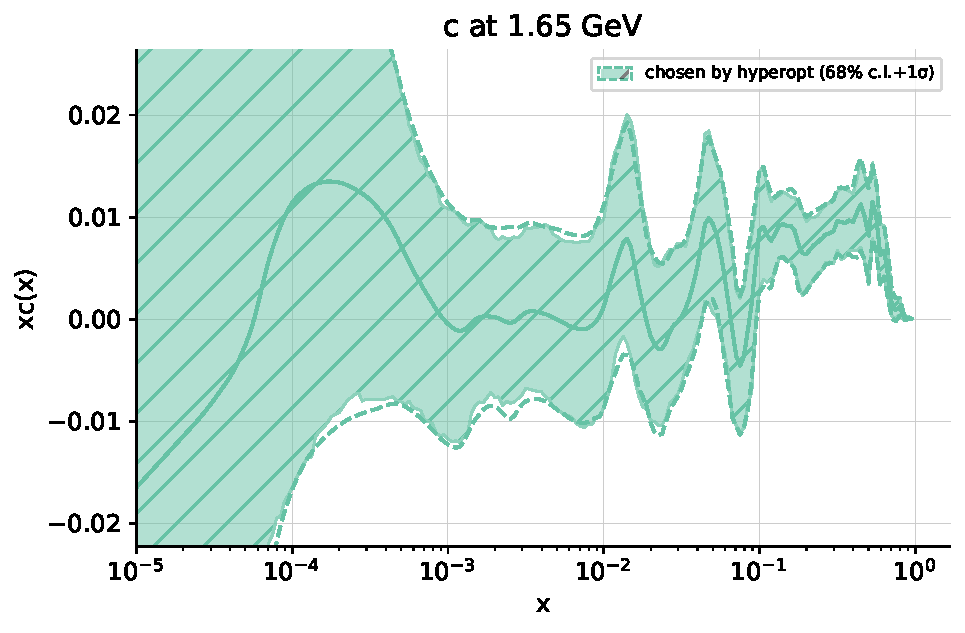
\includegraphics[height=0.45\textheight]{hyperopt_choice_charm_plot_pdfs_c.pdf}\\
      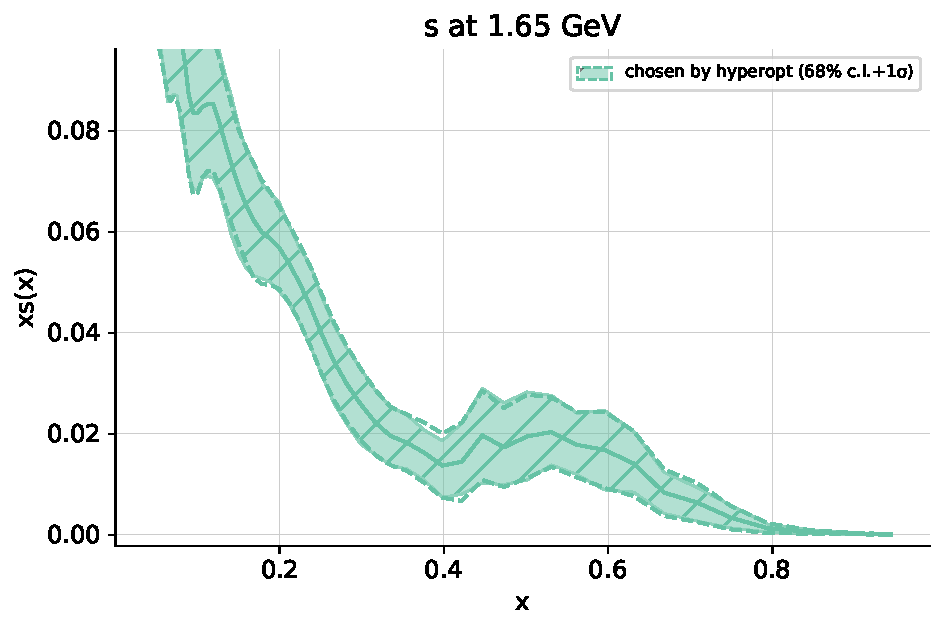
\includegraphics[height=0.45\textheight]{hyperopt_choice_strange_plot_pdfs_s.pdf}
    \end{column}
  \end{columns}
\end{frame}






\section*{A new metric}

\begin{frame}[t]{The idea}

  Ideally, we have an objective metric that is not relative (such as arc-length), but absolute\\\vspace*{1em}

  Correlation between PDFs and validation data suggests overfitting\\\vspace*{1em}

  \textbf{How can we detect when this happens?}
\end{frame}


\begin{frame}[t]{The idea}

  \textbf{Realization: for any PDF the validation loss $\chi^{r}_\text{val}$ should be equal to the ``validation loss'' calculated for any other pseudodata set  $\chi^{\hat{r}}_\text{val}$ (with the same tr/vl mask)}\\\vspace*{1em}

  % For an overfitted PDF we \textbf{expect} $\chi^{r}_\text{val} < \chi^{\hat{r}}_\text{val}$\\\vspace*{1em}

  Thus as a metric for overfitting we might consider
  $$
  \Delta\chi^2_{\text{overfit}}=\langle \chi^{2}_\text{val,$\hat{r}$} - \chi^{2}_\text {val,r}\rangle\quad (<0 \text{ if overfitted})
  $$

  % Though we will need to account for statistical fluctuations:
  % $$ 
  % R_{\text{overfit}}= 
  % \frac{\langle \chi^{\hat{r}}_\text{val} - \chi^{r}_\text {val}\rangle_{\hat{r}}}
  % {\sqrt{\langle ( \chi^{\hat{r}}_\text{val} - \chi^{r}_\text {val}-\langle \chi^{\hat{r}}_\text{val} - \chi^{r}_\text {val}\rangle_{\hat{r}})^2 \rangle_{\hat{r}}}}
  % = \frac{\langle \chi^{\hat{r}}_\text{val} - \chi^{r}_\text {val}\rangle_{\hat{r}}}{\sigma_\text{bootstrap}}
  % $$\\\vspace*{1em}

  While \textbf{underfitted} setups will be filtered due to their higher $\chi^2$ values 

\end{frame}


\section*{Examples}

\begin{frame}[t]{(How) does this work?}

  Let's have a look at a clearly overfitted PDF (preferred by hyperopt):

  \begin{center}
    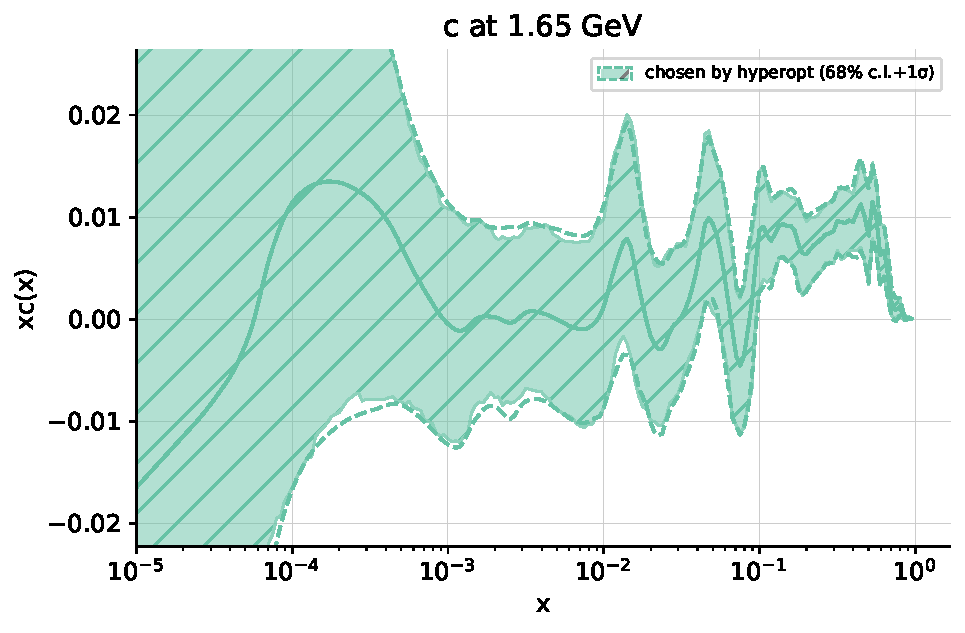
\includegraphics[width=0.4\textwidth]{hyperopt_choice_charm_plot_pdfs_c.pdf}
    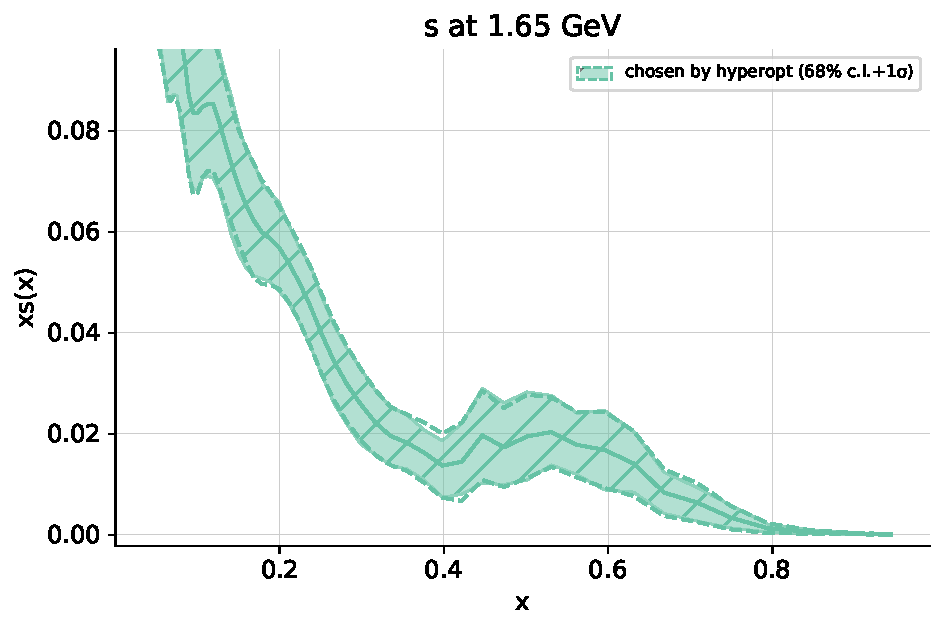
\includegraphics[width=0.4\textwidth]{hyperopt_choice_strange_plot_pdfs_s.pdf}
  \end{center}

  \begin{center}
    $\Delta\chi^2_{\text{overfit}}=-0.0459 \pm 0.0078$ \quad $5.9\sigma$ from 0
  \end{center}
  \textit{The $\Delta\chi^2_{\text{overfit}}$ values and bootstrap errors in these slides are determined using PDFs with $N_{\text{rep}}=100$}

\end{frame}


\begin{frame}[t]{(How) does this work?}

  And now for a PDF that is a bit smoother (ranked \#8 by hyperopt):

  \begin{center}
    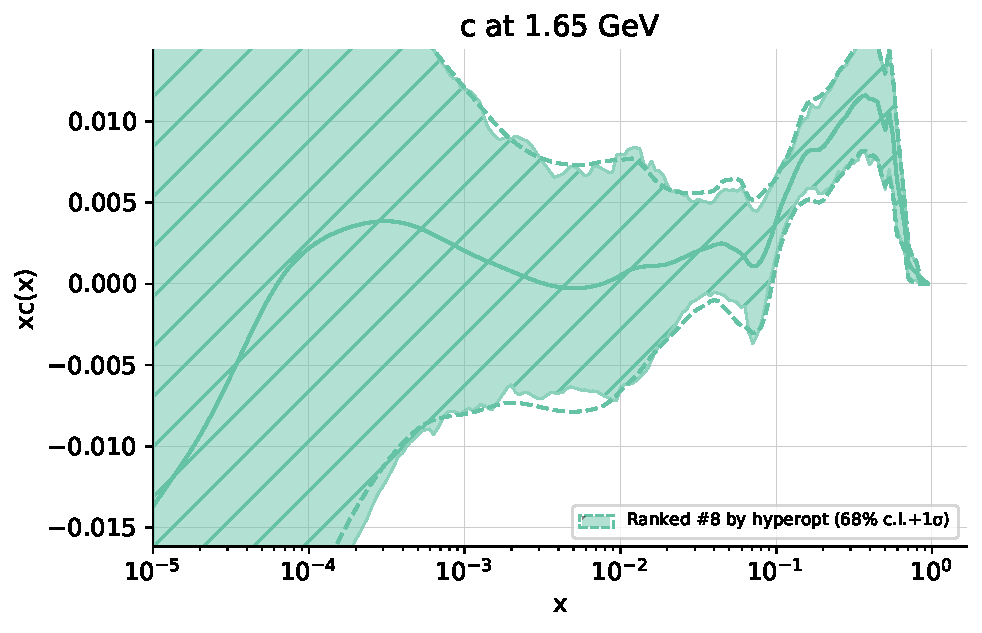
\includegraphics[width=0.4\textwidth]{better_fit_charm_plot_pdfs_c.pdf}
    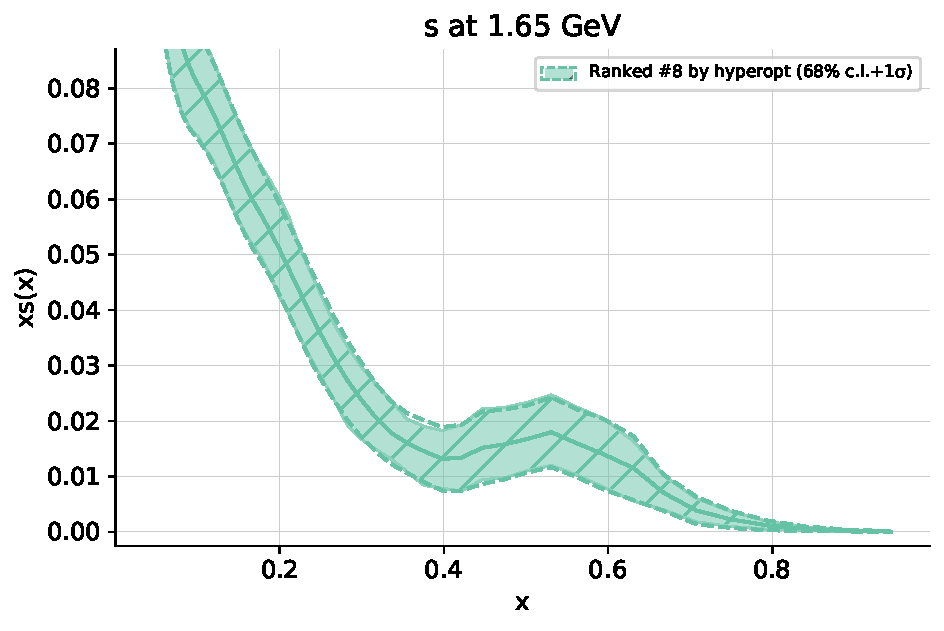
\includegraphics[width=0.4\textwidth]{better_fit_strange_plot_pdfs_s.pdf}
  \end{center}

  \begin{center}
    $\Delta\chi^2_{\text{overfit}}=-0.0168 \pm 0.0105$ \quad $1.6\sigma$ from 0
  \end{center}
  The distance from 0 decreases as expected

\end{frame}


\begin{frame}[t]{(How) does this work?}

  In the past we have had a scenario where this metric would have helped a lot:

  \begin{center}
    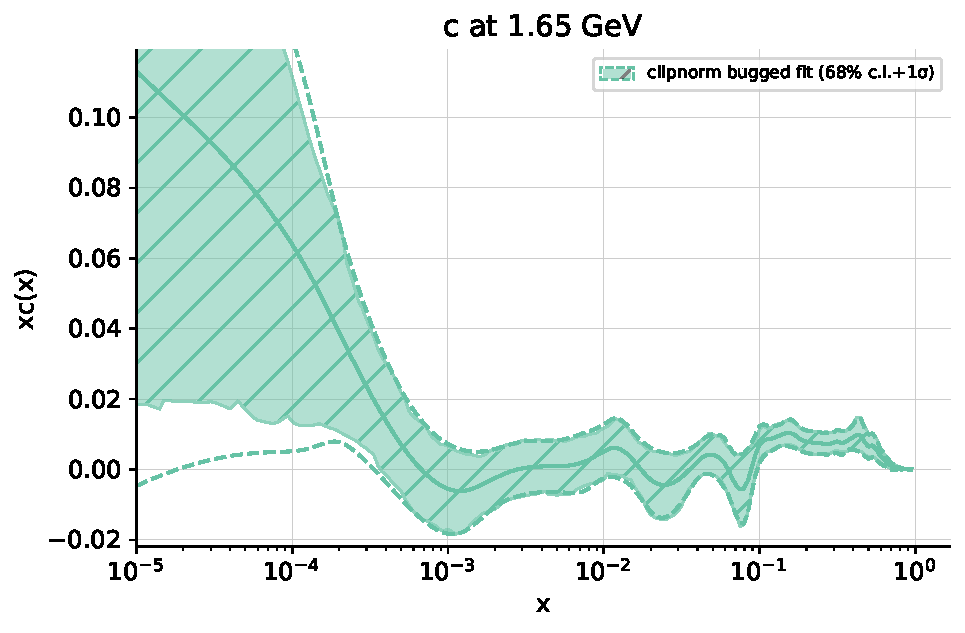
\includegraphics[width=0.4\textwidth]{clipnorm_fit_charm_plot_pdfs_c.pdf}
    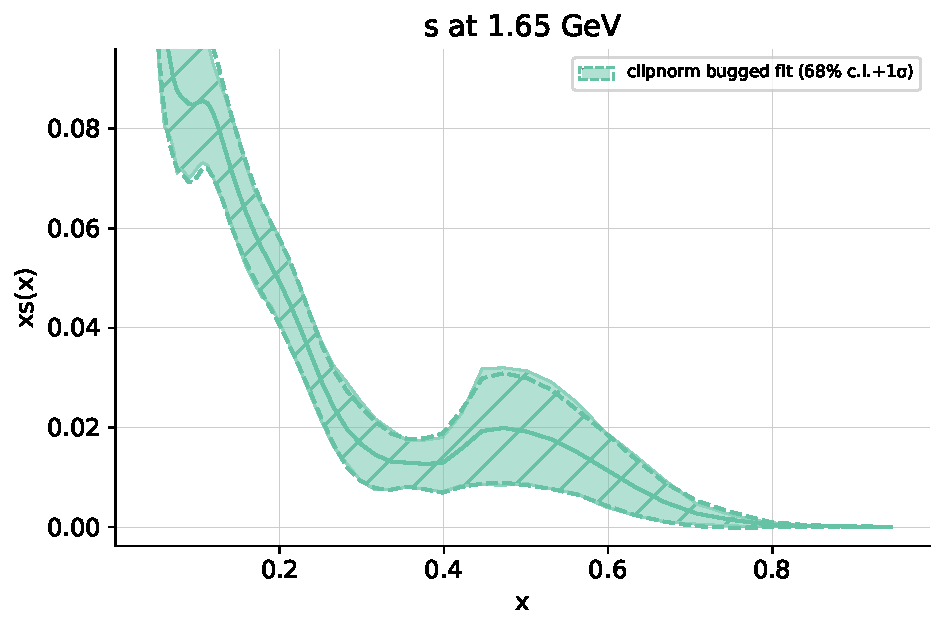
\includegraphics[width=0.4\textwidth]{clipnorm_fit_strange_plot_pdfs_s.pdf}
  \end{center}

  \begin{center}
    $\Delta\chi^2_{\text{overfit}}=-0.0236 \pm 0.0126$ \quad $1.9\sigma$ from 0
  \end{center}

  A clear indicator that the clipnorm bugged fit is overfitted!

\end{frame}


\begin{frame}[t]{(How) does this work?}

  And what about NNPDF4.0?

  \begin{center}
    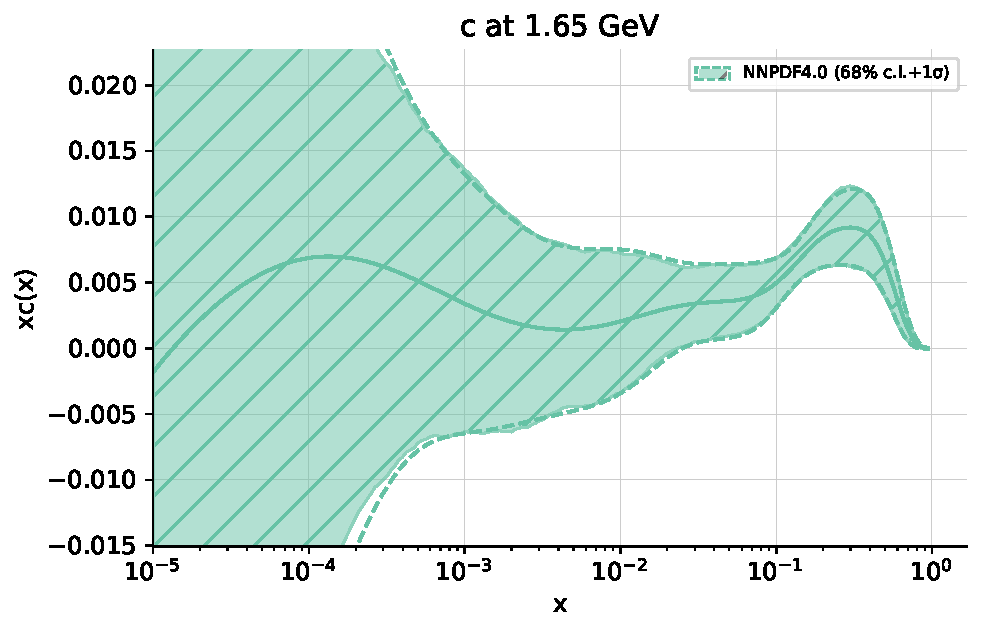
\includegraphics[width=0.4\textwidth]{NNPDF40_fit_charm_plot_pdfs_c.pdf}
    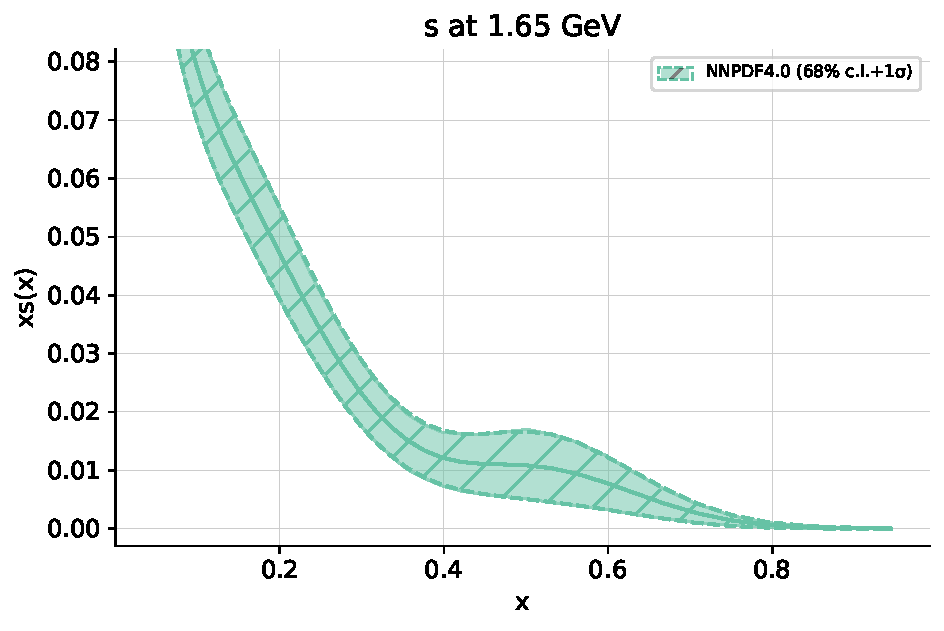
\includegraphics[width=0.4\textwidth]{NNPDF40_fit_strange_plot_pdfs_s.pdf}
  \end{center}

  \begin{center}
    $\Delta\chi^2_{\text{overfit}}=-0.0012 \pm 0.0130$ \quad $0.1\sigma$ from 0
  \end{center}

\end{frame}


\begin{frame}[t]{How can this be used in NNPDF?}

  As an a-posteriory check similar to (but cheaper than) the closure test\\\vspace*{1em}

  \setbeamertemplate{enumerate items}[default]
  \begin{enumerate}
    \item Run hyperoptimization
    \item Select N best setups and do full ~100 replica fits for each
    \item Calculate the estimators for all
    \item Discard setups with e.g. $R_{\text{overfit}} < -1$
    \item
    \begin{enumerate}
      \item Increase number of replicas and repeat...
      \item or select the best of the remaining fit
    \end{enumerate}
  \end{enumerate}\vspace*{1em}

  5.1: If the bootstrap error becomes small enough we will likely always get a negative $\Delta\chi^2_{\text{overfit}}$

  5.2: What is an acceptable $\Delta\chi^2_{\text{overfit}}$? \\
  \qquad How do we define the best fit ($\chi^2_{\text{val}}$, $\chi^2_{\text{tr}}$, $\chi^2_{\text{exp}}$, \ldots)?\\\vspace*{1em}

  \only<1>{\color{white}Conclusion: The $\Delta\chi^2_{\text{overfit}}$ provides a metric for overfitting that can be used to flag overfitted hyperparameter setups and thereby reduce human bias}
  \only<2>{Conclusion: The $\Delta\chi^2_{\text{overfit}}$ provides a metric for overfitting that can be used to flag overfitted hyperparameter setups and thereby reduce human bias}
\end{frame}



\begin{frame}{Determination of the photon PDF}
  \begin{columns}[T]
    \begin{column}{0.59\textwidth}
      Initially the photon PDF has been determined in different ways:
      \begin{itemize}
        \item physical model: sensitive to underlying model
        \item fitting: data does not provide strong constraints
      \end{itemize}

      \vspace*{0.5em}
      However with the LUXqed approach it can be computed perturbatively \\
      based on the observation that the heavy-lepton production cross-section can be written in two ways:
      \begin{itemize}
        \item in terms of structure functions $F_2$, $F_L$
        \item in terms of PDFs (including the photon)
      \end{itemize}

      \vspace*{0.5em}
      luxQED result {\color{gray}\small[Manohar, Nason, Salam, Zanderighi: 1607.04266, 1708.01256]}:
      \vspace*{-0.8em}
      \begin{equation*}
        \begin{split}
          & x \gamma(x, \mu^2)
          =
          \frac{2}{\alpha (\mu^2)} \int\limits_x^1 \frac{dz}{z}
          \Biggl\{ \int_{m_p^2x^2 \over 1-z}^{\mu^2 \over 1-z} \frac{dQ^2}{Q^2}
          \alpha^2(Q^2) \Biggl[ -z^2 F_L(x/z, Q^2) \\
          & + \left( z P_{\gamma q}(z) + \frac{2 x^2 m_p^2}{Q^2} \right)
          F_2(x/z, Q^2)\Biggr] - \alpha^2(\mu^2) z^2 F_2(x/z, \mu^2)\Biggr\}
        \end{split}
      \end{equation*}
    \end{column}

    \begin{column}{0.39\textwidth}
      \vspace*{-2.5em}
      \begin{figure}
        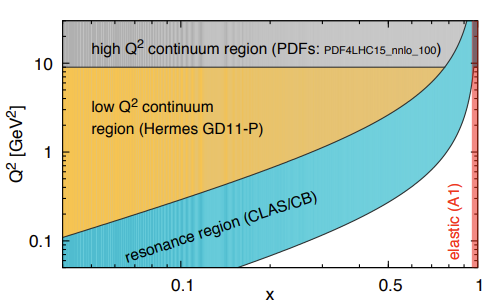
\includegraphics[width=0.89\textwidth]{figures/dataluxqed.png}
        \caption*{Input to construct $F_2$ and $F_L$}
        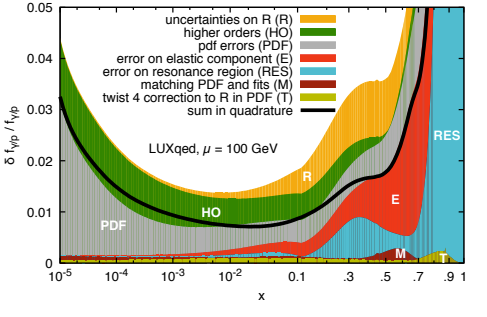
\includegraphics[width=0.89\textwidth]{figures/luxQED_uncs.png}
        \caption*{Sources of uncertainty}
      \end{figure}
    \end{column}
  \end{columns}
\end{frame}


\begin{frame}{LUXqed PDF determinations}
  LUXqed has been used in all of the most recent QED PDFs:
  \begin{itemize}
      \item LUXqed\_plus\_PDF4LHC15 {\color{gray}\small [1607.04266]}
      \item LUXqed17\_plus\_PDF4LHC15 {\color{gray}\small [1708.01256]}
      \item MMHT2015qed {\color{gray}\small [1907.02750]}
      \item NNPDF3.1luxQED {\color{gray}\small [1712.07053]}
      \item CT18lux and CT18qed {\color{gray}\small [2106.10299]}
      \item MSHT20QED {\color{gray}\small [2111.05357]}
      \item MSHT20qed\_an3lo {\color{gray}\small [2312.07665]}
      \item NNPDF4.0QED {\color{gray}\small [2401.08749 ]}
  \end{itemize}
\end{frame}

% \begin{frame}{Results: photon PDF and luminosity}
%   \begin{center}
%     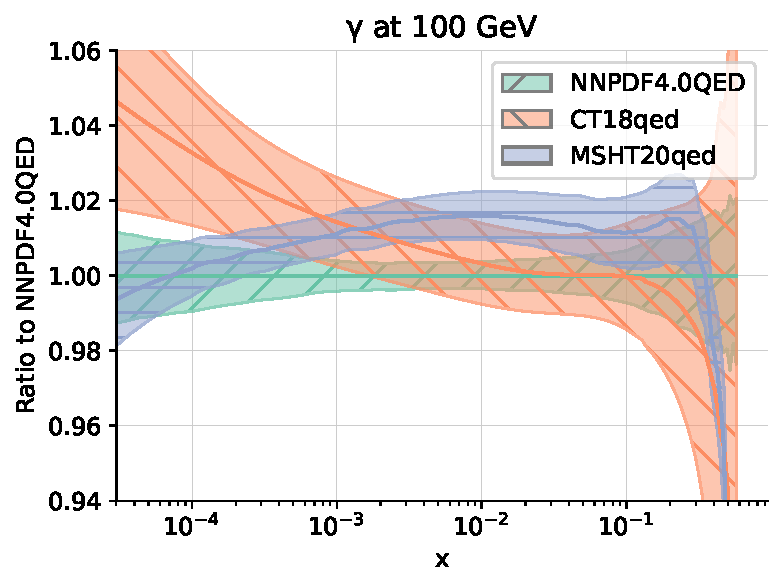
\includegraphics[width=0.3\textwidth]{figures/photon_comparison.pdf}
%     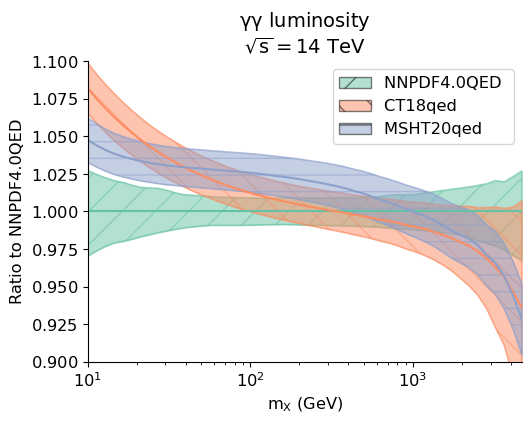
\includegraphics[width=0.3\textwidth]{figures/pp_lumi_comparison.png}
%     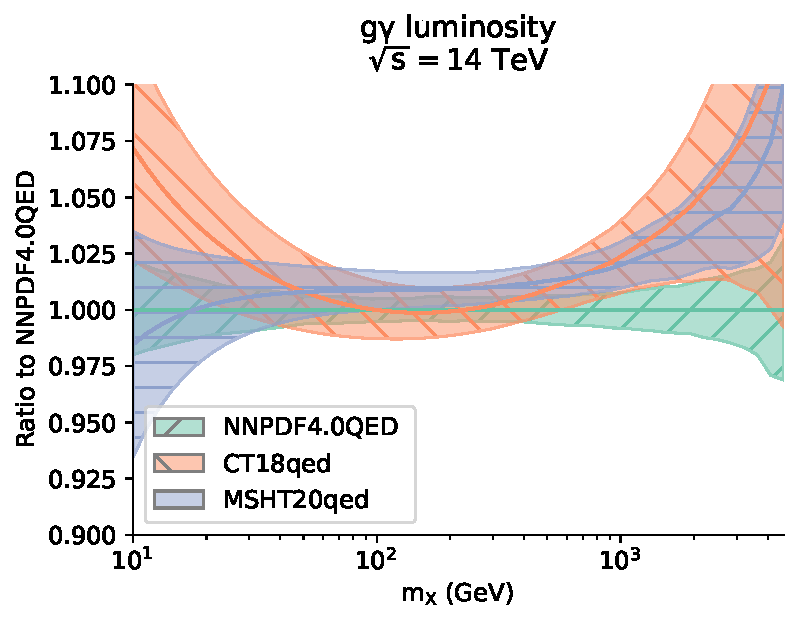
\includegraphics[width=0.3\textwidth]{figures/gp_lumi_comparison.pdf}
%   \end{center}
%   \begin{itemize}
%     \item Because all groups use the luxQED formalism, the photon PDFs agree at percent level
%     \item Luminosity generally in agreement, but differ at very small and very large invariant mass
%   \end{itemize}
% \end{frame}


% ============================================================================


\begin{frame}{Incomplete higher order uncertainties covmat}
  \begin{itemize}
    \item We construct an IHOU matrix following a similar approach by varying the subleading functions
    \item IHOU are independent of MHOU so the uncertainties are added in quadrature
    $$C = C_\mathrm{exp}+C_\mathrm{MHOU}+C_\mathrm{IHOU}$$
  \end{itemize}

  \begin{columns}
    \begin{column}{0.49\textwidth}
      \begin{figure}[!t]
        \centering
        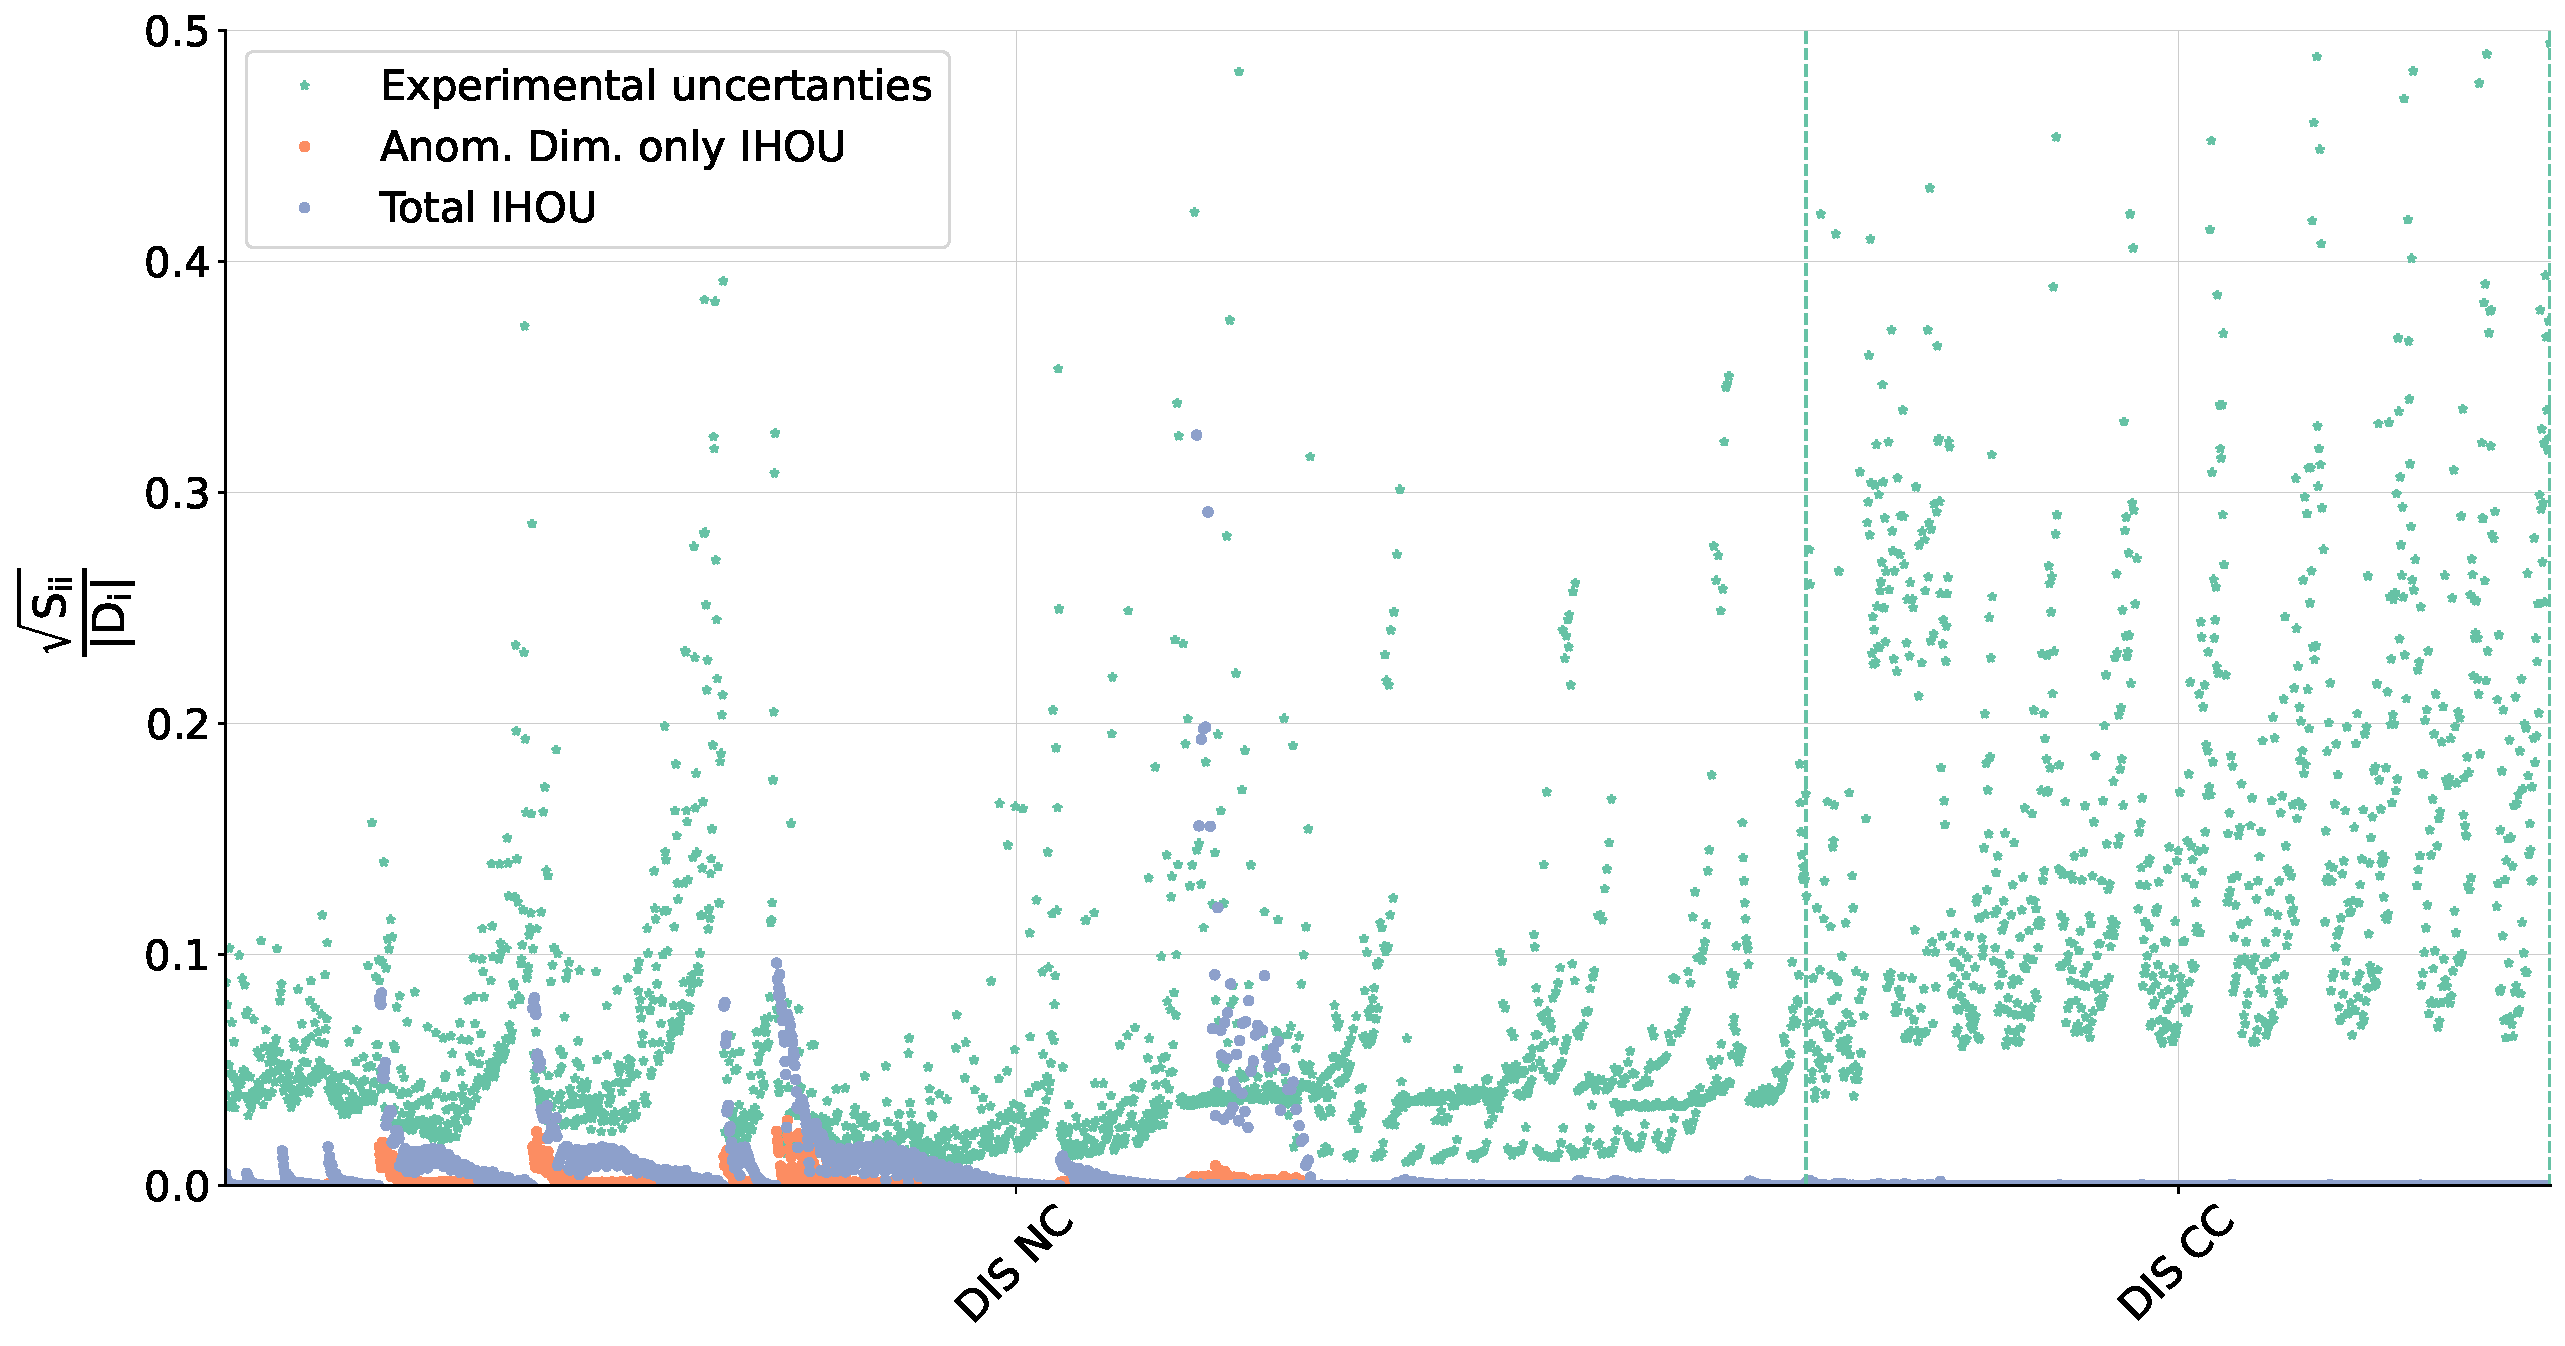
\includegraphics[width=.9\textwidth]{figures/diag_cov_dis_ihou.pdf}
        \caption*{IHOU have a large effect on small-$x$, low-$Q$ DIS data
        }
      \end{figure}
    \end{column}
    \begin{column}{0.49\textwidth}
      \begin{figure}[!t]
        \centering
        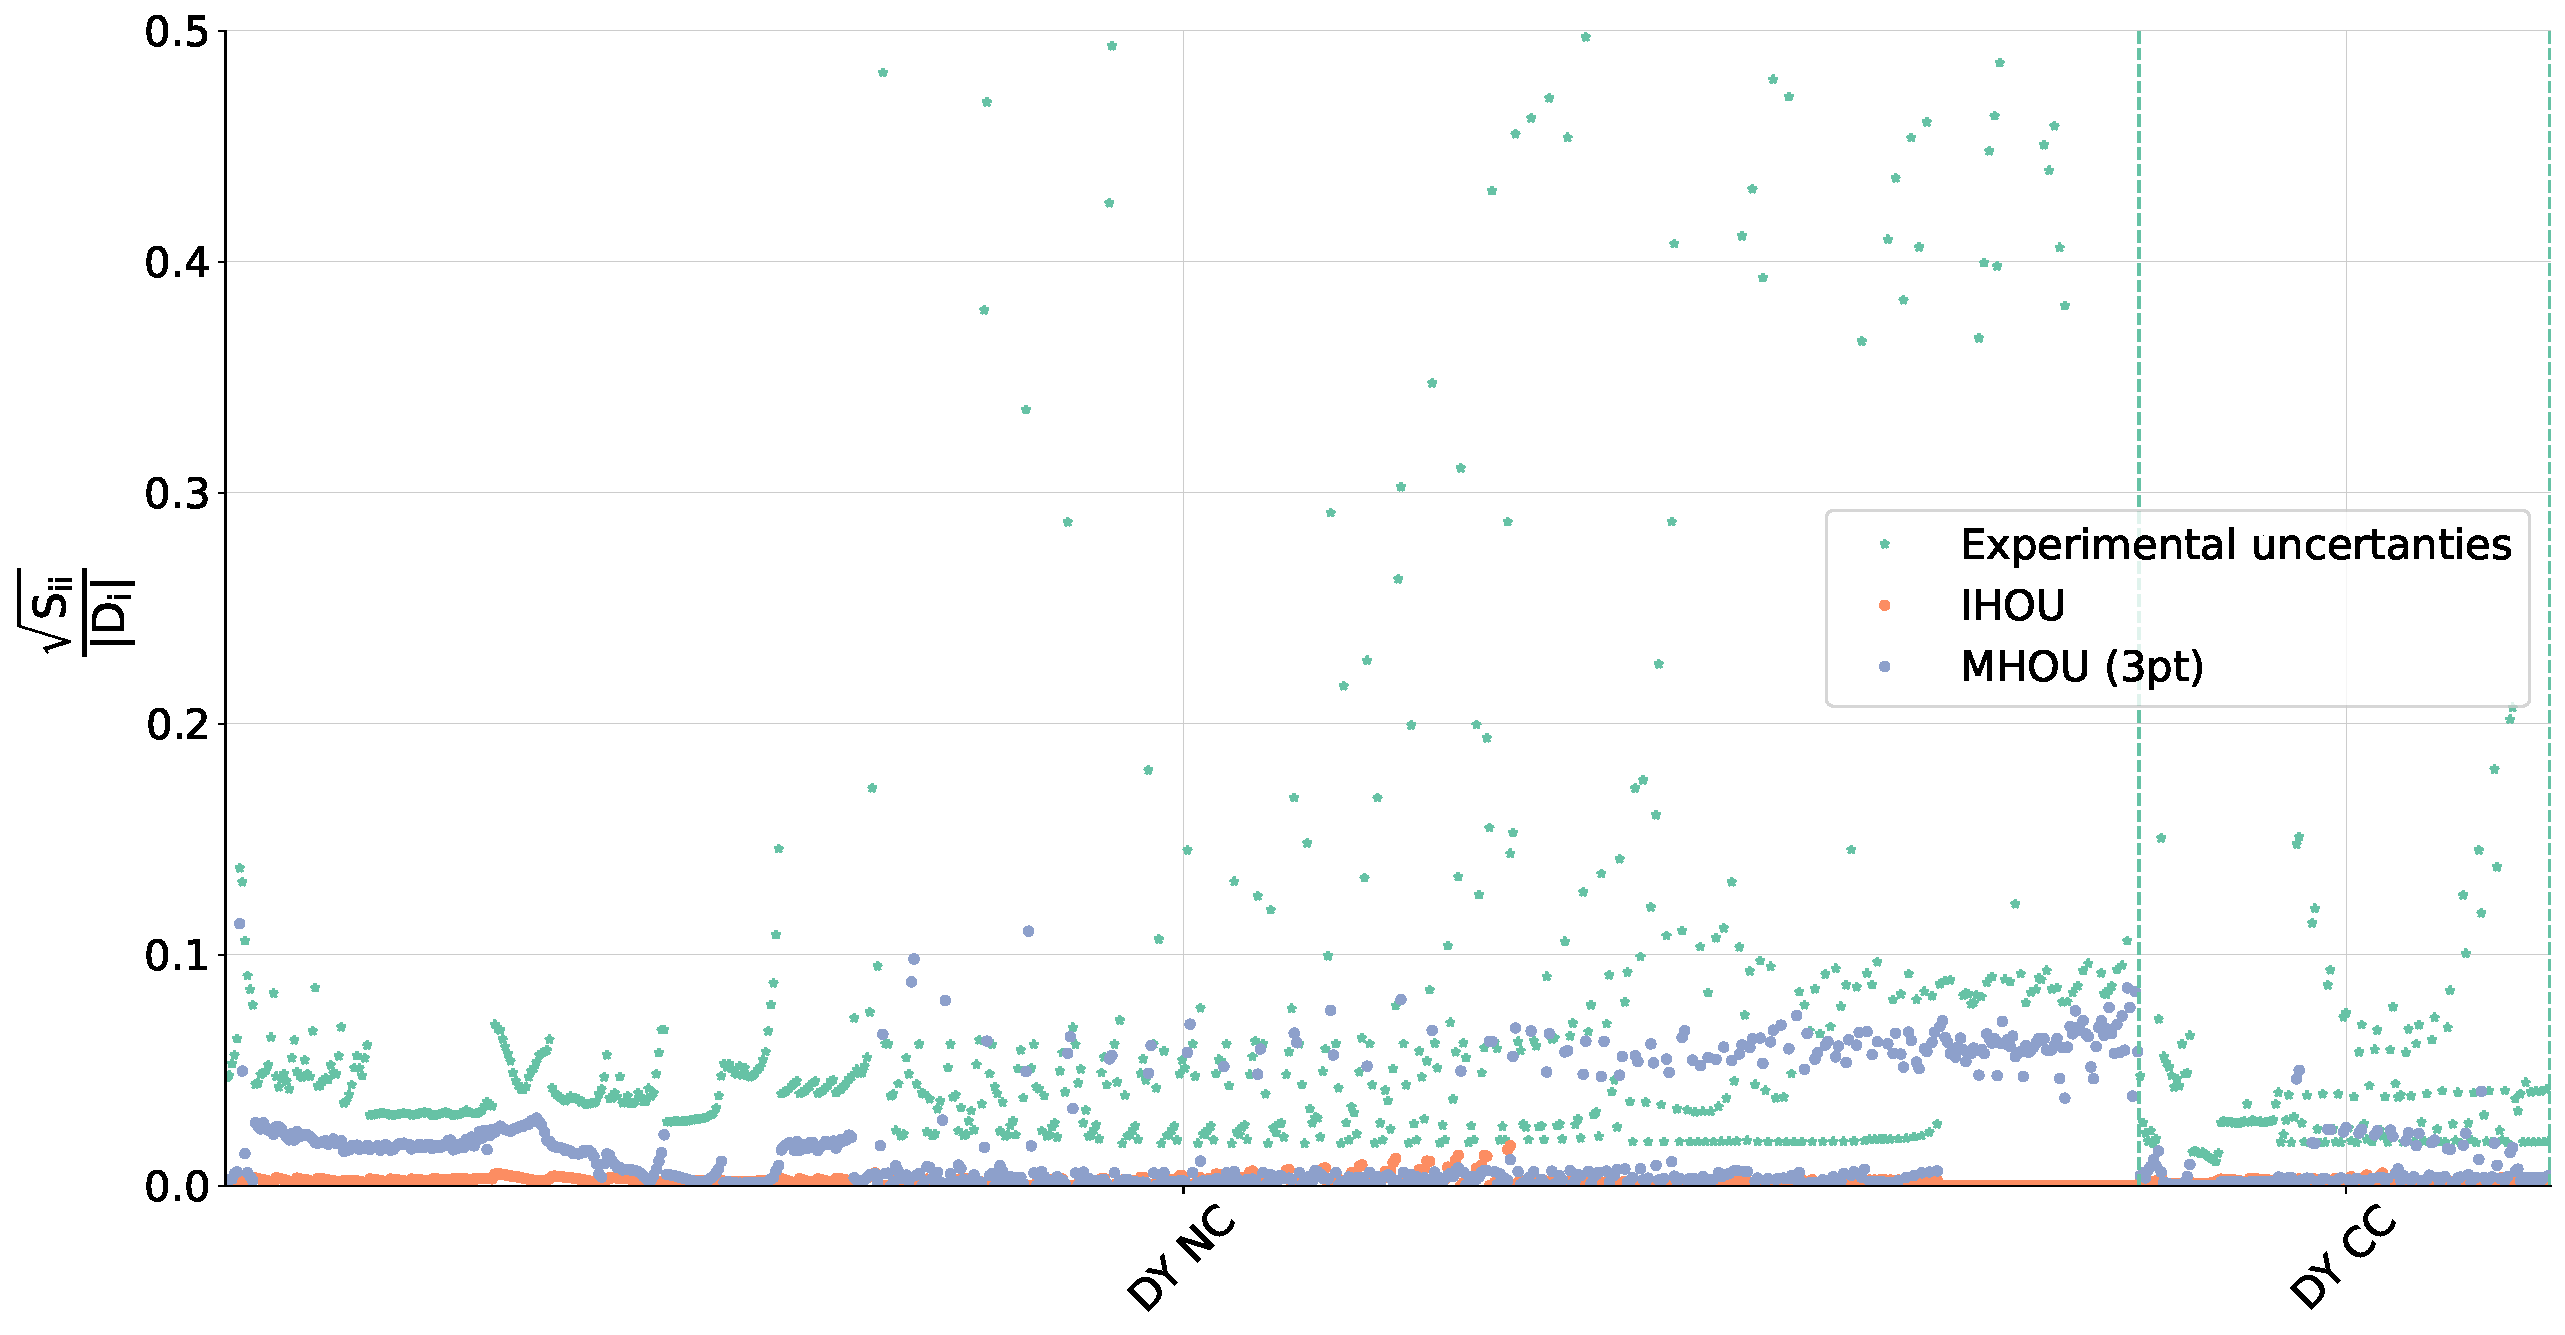
\includegraphics[width=.9\textwidth]{figures/diag_cov_dy_ihou_3pt_mhou.pdf}
        \caption*{NNLO MHOU included where N3LO not available \\
          MHOU can similar magnitude as the experimental uncertainty
        }
      \end{figure}
    \end{column}
  \end{columns}


\end{frame}

% \begin{frame}{Magnitude of theory uncertainties}
% % show that for certain processes th unc is of same size as exp unc.
% \end{frame}

% ============================================================================

\begin{frame}{Impact of MHOUs at N3LO}
  \begin{figure}[!t]
    \centering
    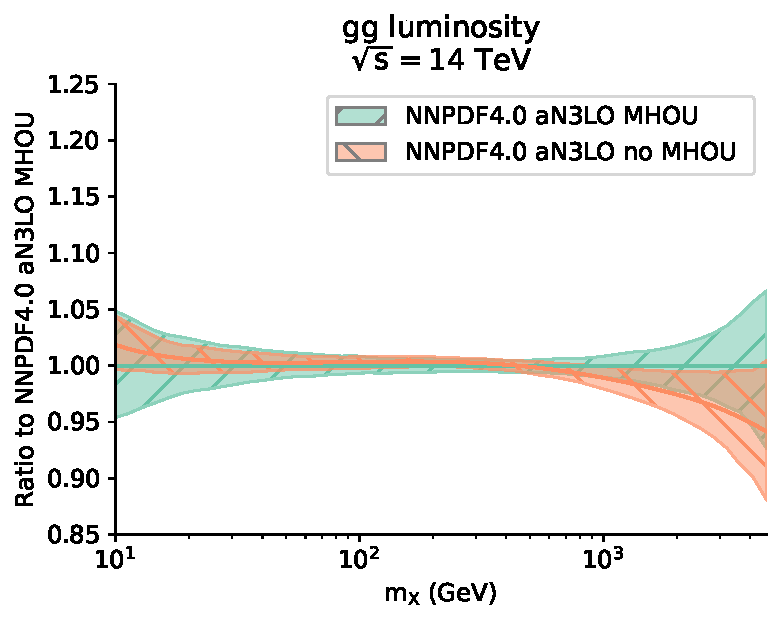
\includegraphics[width=0.45\textwidth]{figures/gg_plot_lumi1d.pdf}
    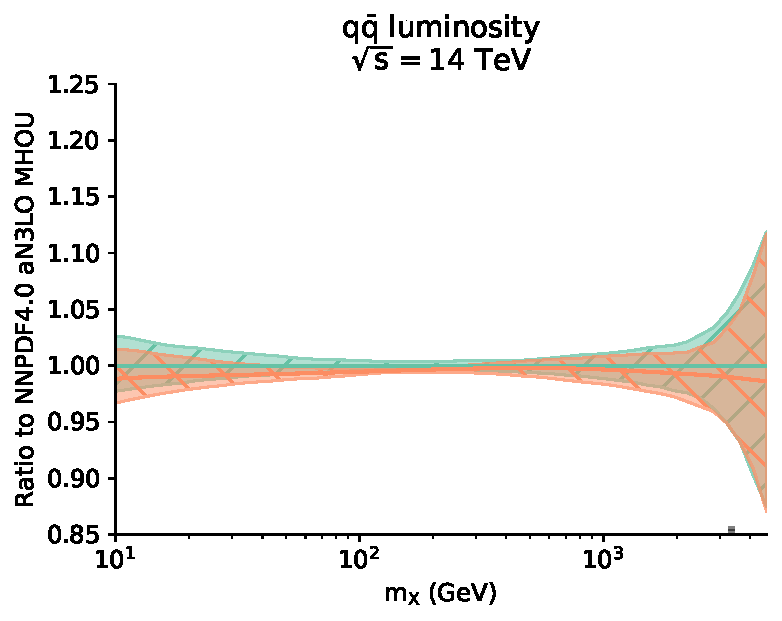
\includegraphics[width=0.45\textwidth]{figures/qqbar_plot_lumi1d.pdf}
  \end{figure}
  \begin{itemize}
    \item Non-negligible impact of MHOUs even at N3LO
    \item[$\Rightarrow$] reason to include exact N3LO calculations for hadronic processes
  \end{itemize}
\end{frame}


% \begin{frame}{Comparison to MSHT20}
%   \begin{figure}[!t]
%     \centering
%     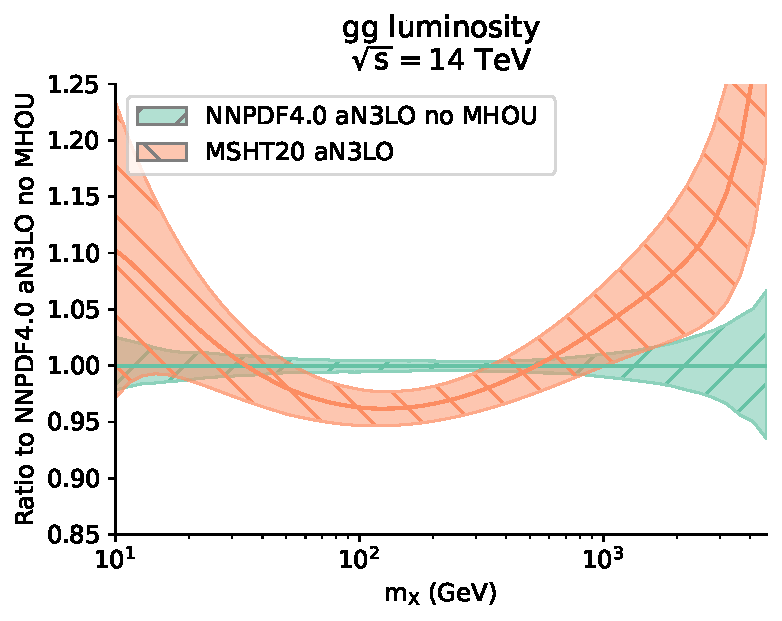
\includegraphics[width=0.45\textwidth]{figures/gg_plot_lumi1d_msht20.pdf}
%     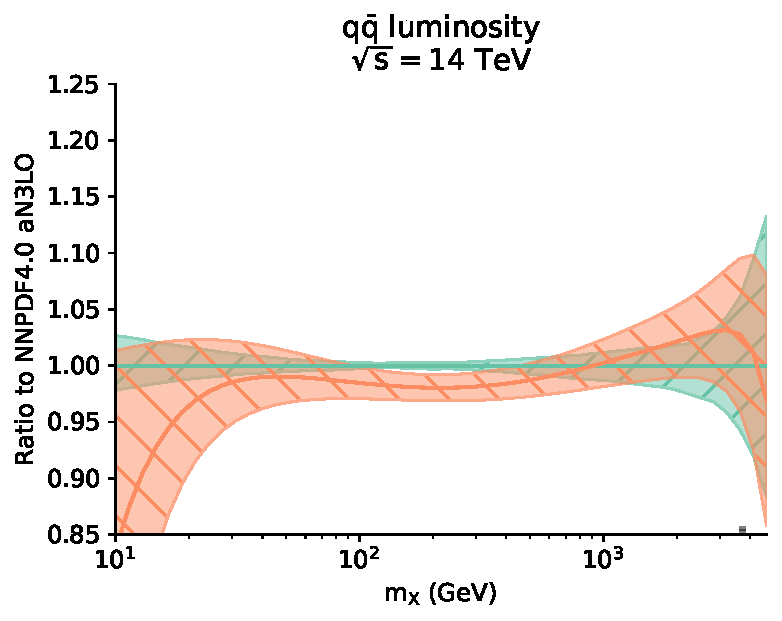
\includegraphics[width=0.45\textwidth]{figures/qqbar_plot_lumi1d_msht20.pdf}
%   \end{figure}
%   \begin{itemize}
%     \item Good agreement with MSHT20 for the quark luminosities
%     \item Also for gluon luminosities, except around the Higgs mass and high-mass
%     \item Similar data but different methodology (including splitting function parametrization)
%   \end{itemize}
% \end{frame}



\end{document}
